\chapter{RESULTS AND ANALYSIS}
The Automated Nutrient Dosing and Monitoring System, at the current level of its development, collects the data of pH, TDS, temperature, and humidity sensors and presents it on a web-based dashboard. The sensors are linked to the ESP32 microcontroller, which monitors real time environmental and nutrient variables of the hydroponic system. The ESP32 sends this sensor data to a cloud database via the Wi-Fi connection, where the readings are stored in a cloud database together with timestamps.
\\[10pt]
The data is then stored and can be accessed and displayed on the web dashboard so that users can monitor pH, nutrient concentration, temperature and humidity. The dashboard presents both live values and graphical trends, confirming that sensor data acquisition, wireless communication, database storage, and frontend visualization are working correctly. These results demonstrate that the system is able to reliably sense, transmit, store, and display hydroponic parameters in real time. Users can also update threshold values to suit different crops.
\begin{figure}[H]
    \centering
    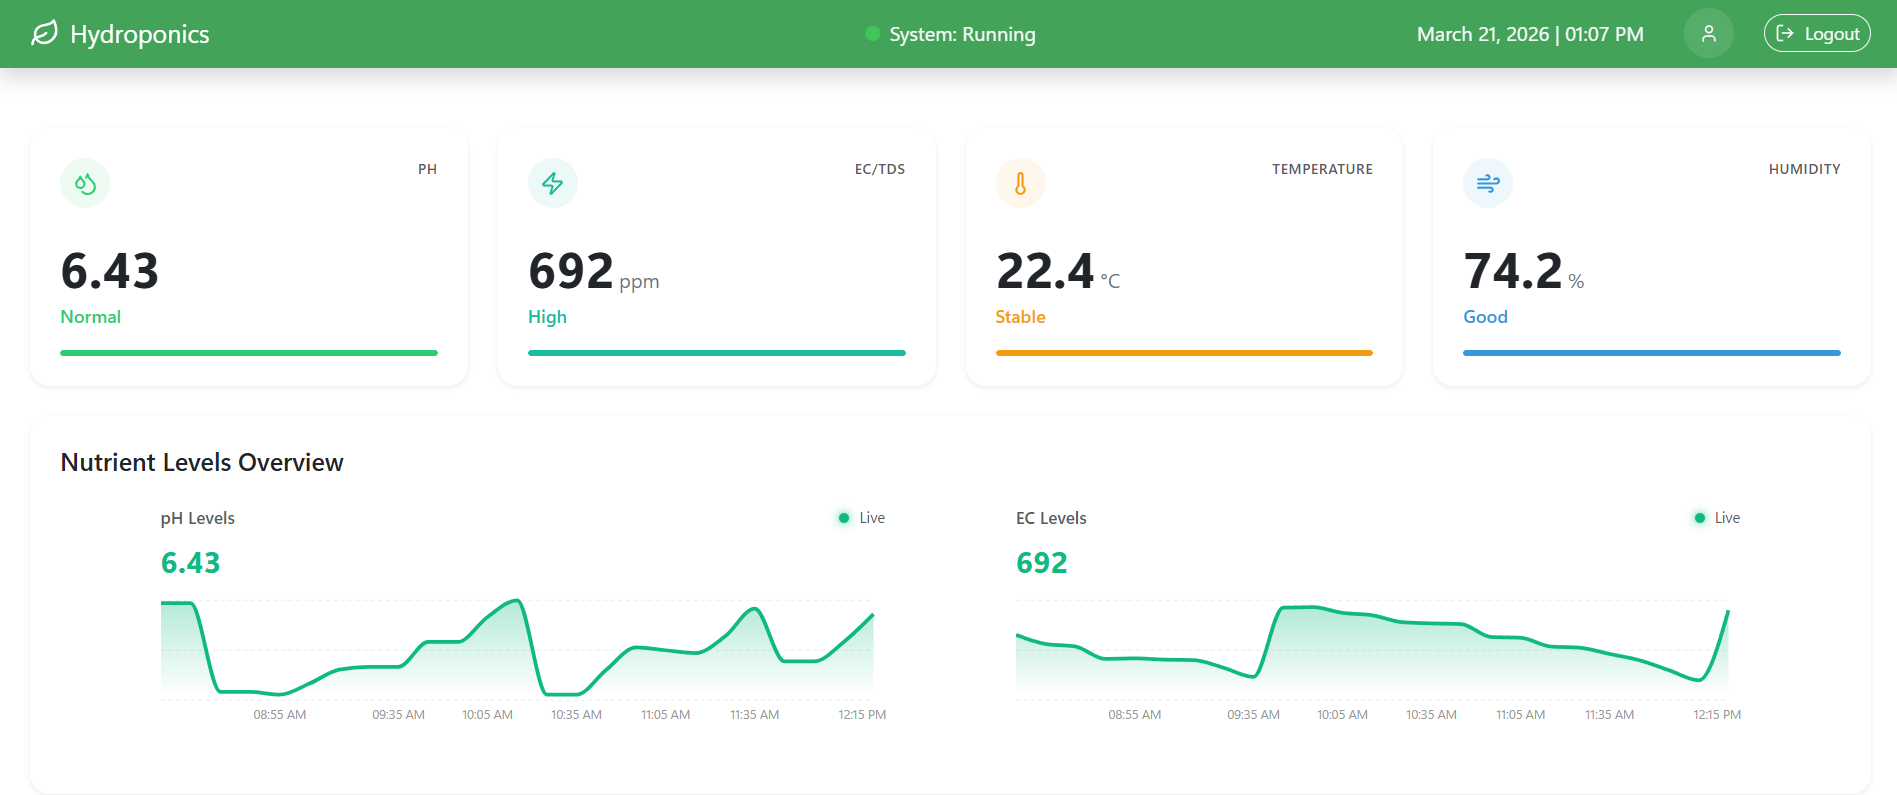
\includegraphics[width=1\linewidth,height=7cm]{src/images/dashboard.png}
    \caption{Screenshot of dashboard with current data graphs}
    \label{fig: dashboard}
\end{figure}

The plant configuration page serves as the primary control interface through which operators define and update the crop-specific setpoints that control the automated dosing behaviour of the system. The interface is accessible through the web-based dashboard and communicates with the backend server via RESTful API calls, which updates the values to the ESP32 microcontroller through the cloud database. At the top of the page, the active plant profile is displayed as Lettuce, confirming that the system is currently operating under lettuce-specific parameter ranges. The plant selection dropdown allows the operator to switch between preconfigured crop profiles, each of which carries its own recommended thresholds for pH, EC/TDS, and humidity, enabling the system to be repurposed for different crops without requiring firmware modifications.\\[10pt]
\begin{figure}[H]
    \centering
    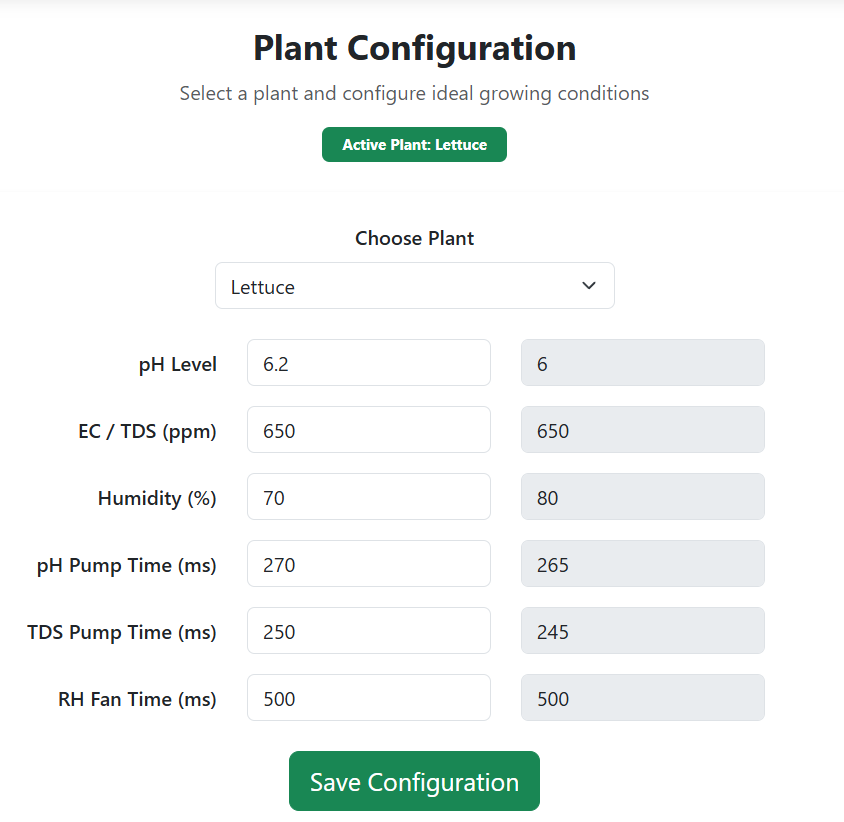
\includegraphics[width=1\linewidth]{src/images/configuration.png}
    \caption{Plant parameters configuration}
    \label{fig: PlantCalibration}
\end{figure}
Once the operator clicks Save Configuration, the updated values are written to the Supabase cloud database, from which the ESP32 firmware fetches them at the end of each monitoring cycle as defined in the control loop. This architecture ensures that parameter updates take effect at the next scheduled dosing check without interrupting the ongoing monitoring process, maintaining system continuity during configuration changes and providing remote access.\\[10pt]
Error was observed on ESP pins GPIO4 (ADC1\_CH3) and GPIO2 (ADC2\_CH3) while reading analog data during testing where garbage values were observed possibly due to stray capacitances in the prototype board. GPIO2 and GPIO4 are also essential for boot functions i.e. LOW/HIGH at boot, and bootstrapping respectively. Whenever WiFi or Bluetooth is enabled, the aforementioned pins generally referred to as ADC2 pins are taken over by the RF subsystem and are regarded as unstable for analog readings, thus they return garbage values or fail.
Therefore pins ESP32 GPIO34 (ADC1\_CH6), GPIO35 (ADC1\_CH7), and GPIO32 pins were used for pH, TDS, and DHT22 analog data inputs respectively.

\begin{figure}[H]
    \centering
    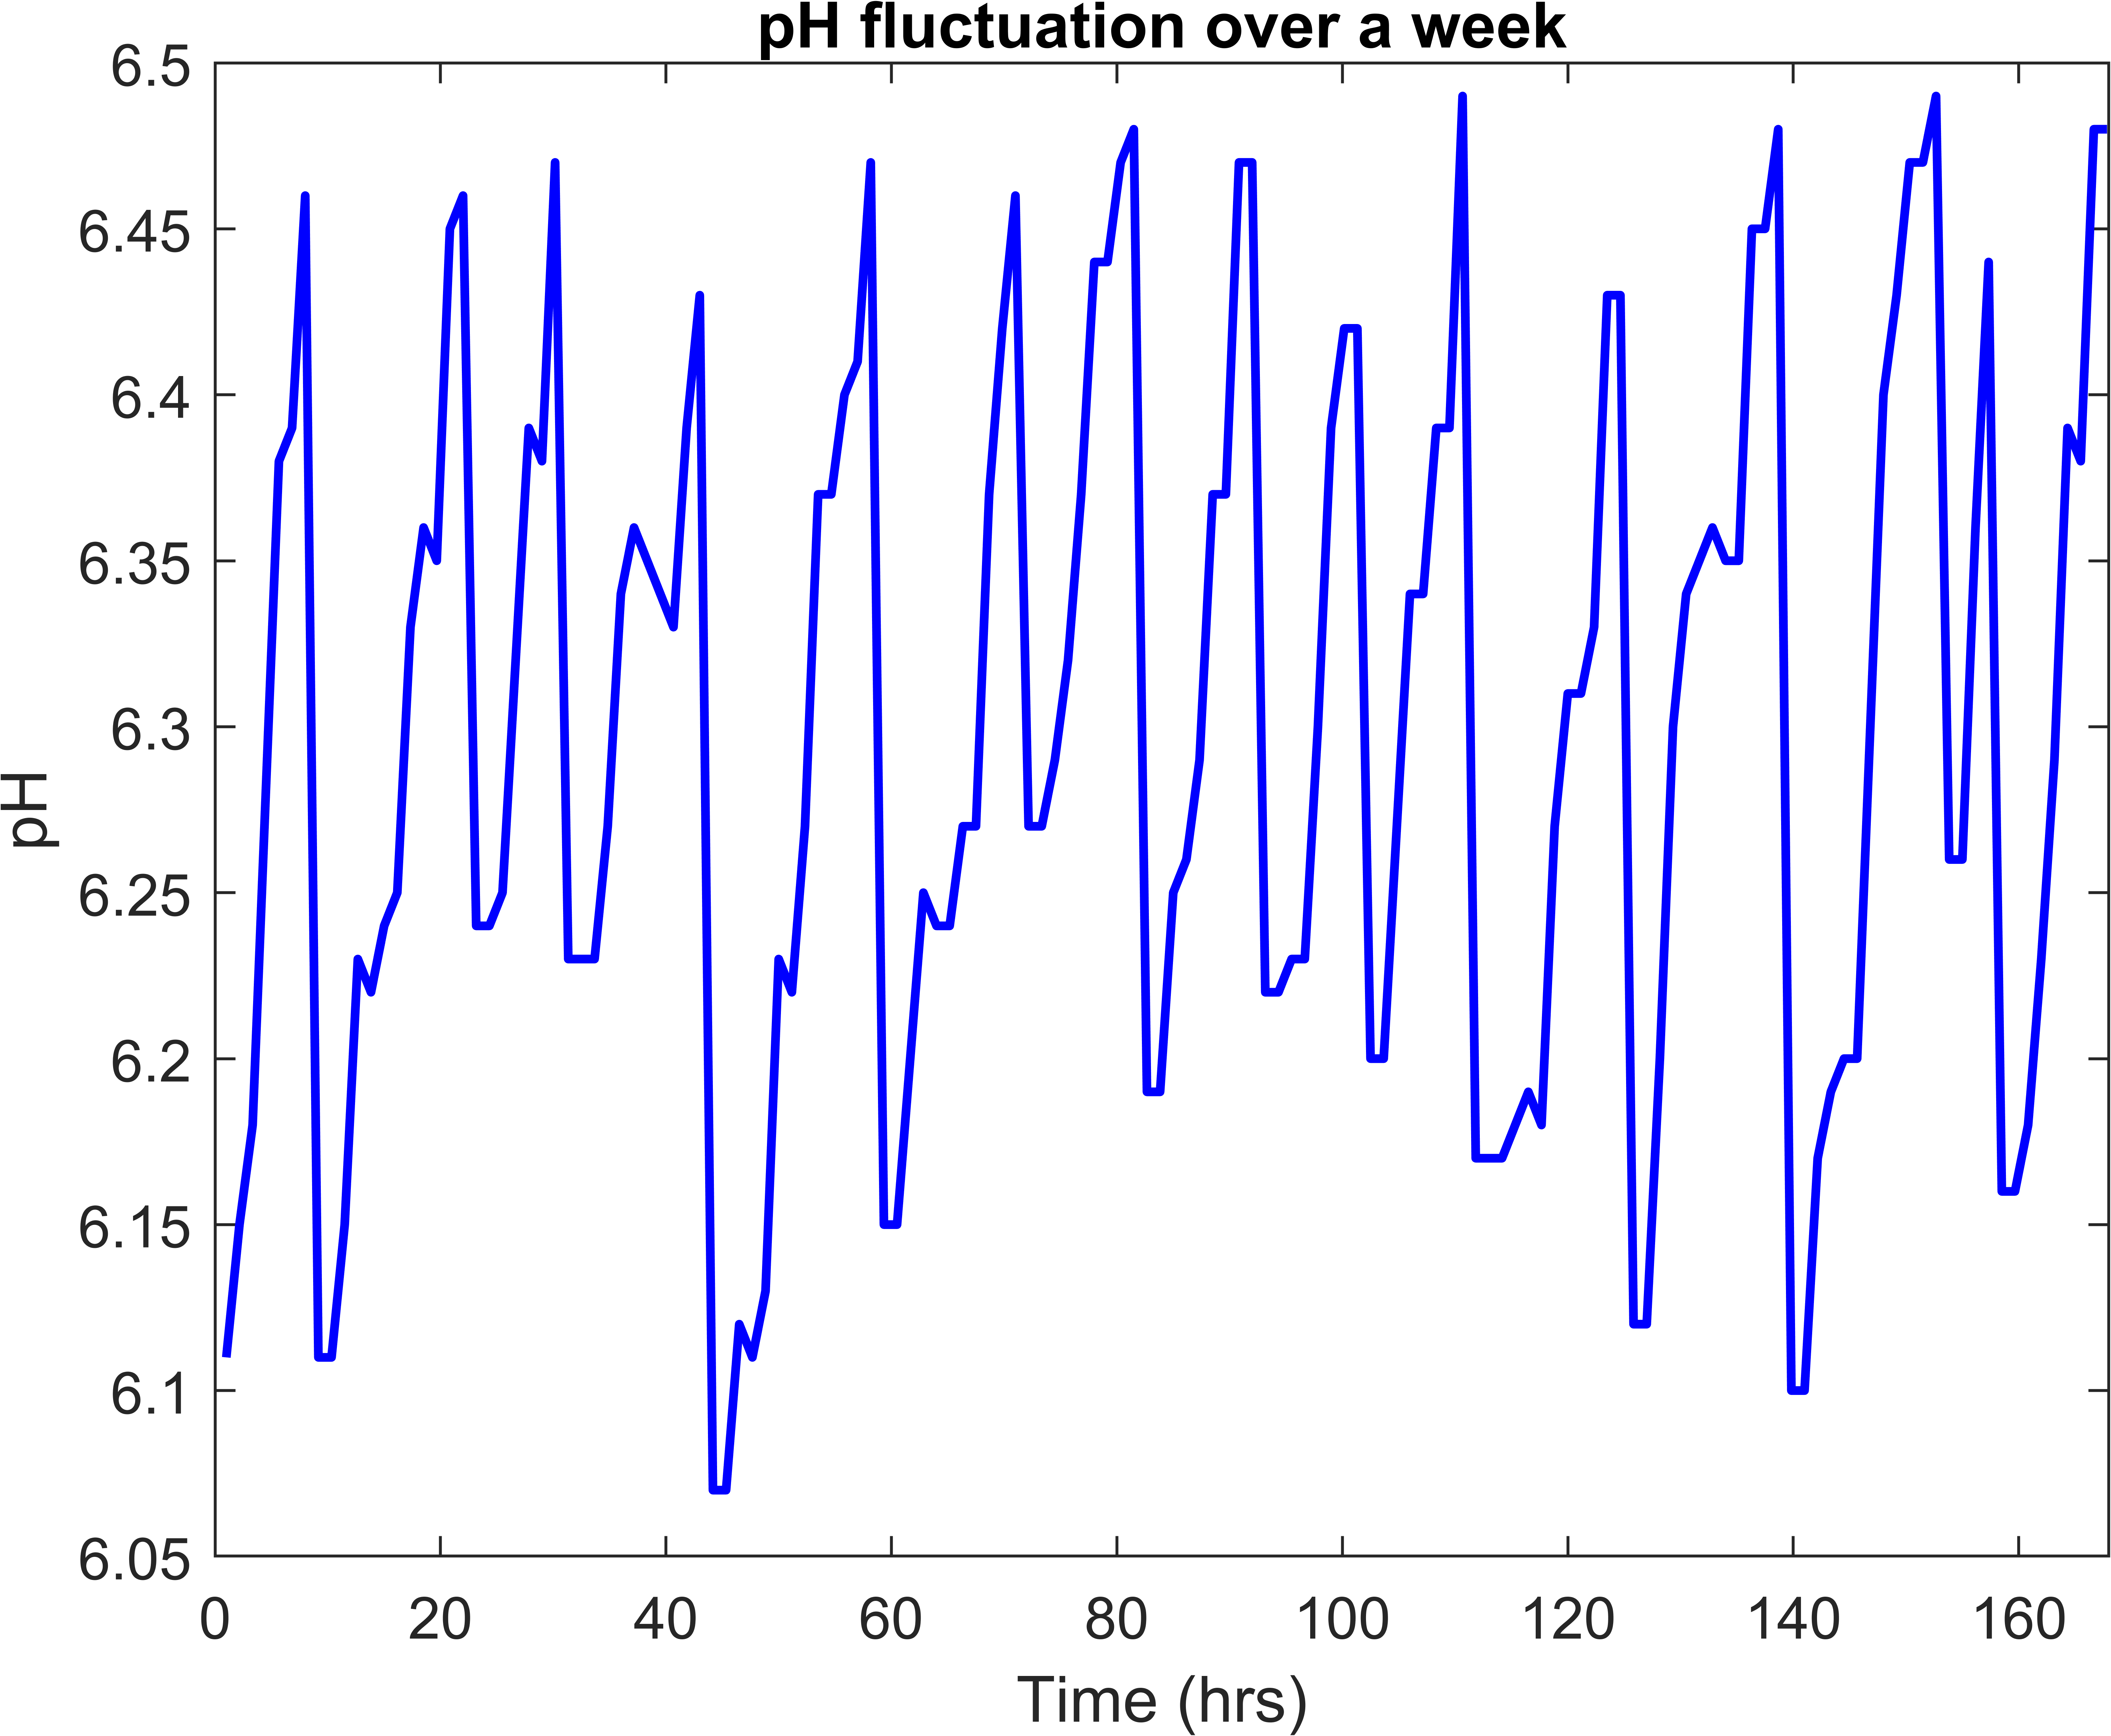
\includegraphics[width=0.8\linewidth]{src/images/phGraph.png}
    \caption{pH Fluctuation Graph over a week}
    \label{fig: phGraph}
\end{figure}

The pH fluctuation graph recorded over 1 week (168-hour period) demonstrates the closed-loop control system working consistently within the optimal range of 6.0 to 6.5 for lettuce cultivation. The actual range for lettuce is 5.5 to 6.5 pH but the lower threshold of 6.0 pH was kept to avoid overdosing. Through the data, we can observe a recurring sawtooth pattern throughout the entire week, which is characteristic of threshold-based control. In each cycle, pH rises gradually due to the absorption of anions such as nitrate and phosphate by the lettuce roots as a result of nutrient dosing, which progressively alkalises the solution. Once pH reaches the upper threshold of 6.5, the acid dosing pump is turned, delivering a measured quantity of pH-down solution that brings the value back down to approximately 6.1 to 6.2, after which the natural gradual upward drift can be seen again after the observed sharp drop due to adding acidic pH balancing solution.
The amplitude of each cycle remains consistent at approximately $\pm$0.30--0.38 pH units, and the correction response is applied reliably across all seven days without any instance of the value crossing the defined boundaries. The system did not require pH up dosing at any point during the observation period, which aligns with expected behaviour since lettuce systems under normal operating conditions tend to alkalise rather than acidify the solution. These results confirm that the pH regulation subsystem is working correctly and maintaining solution chemistry within the crop-specific tolerance band.
Since the pH meter used was not a continuous measurement industrial grade equipment, the pen-type commercial pH meter had to be recalibrated rather frequently due to deviation from true pH value reflected by a spare pen-type pH meter. To mitigate inaccuracies and accidental dosing due to inaccurate pH readings, the pH meter continually submerged in the solution was recalibrated with given buffer solutions every 4 days. Along with recalibration, new values of the interpolated $MID\_PH_{7}$ had to be calculated since the measured electrode potentials were also observed to deviate. 

\begin{figure}[H]
    \centering
    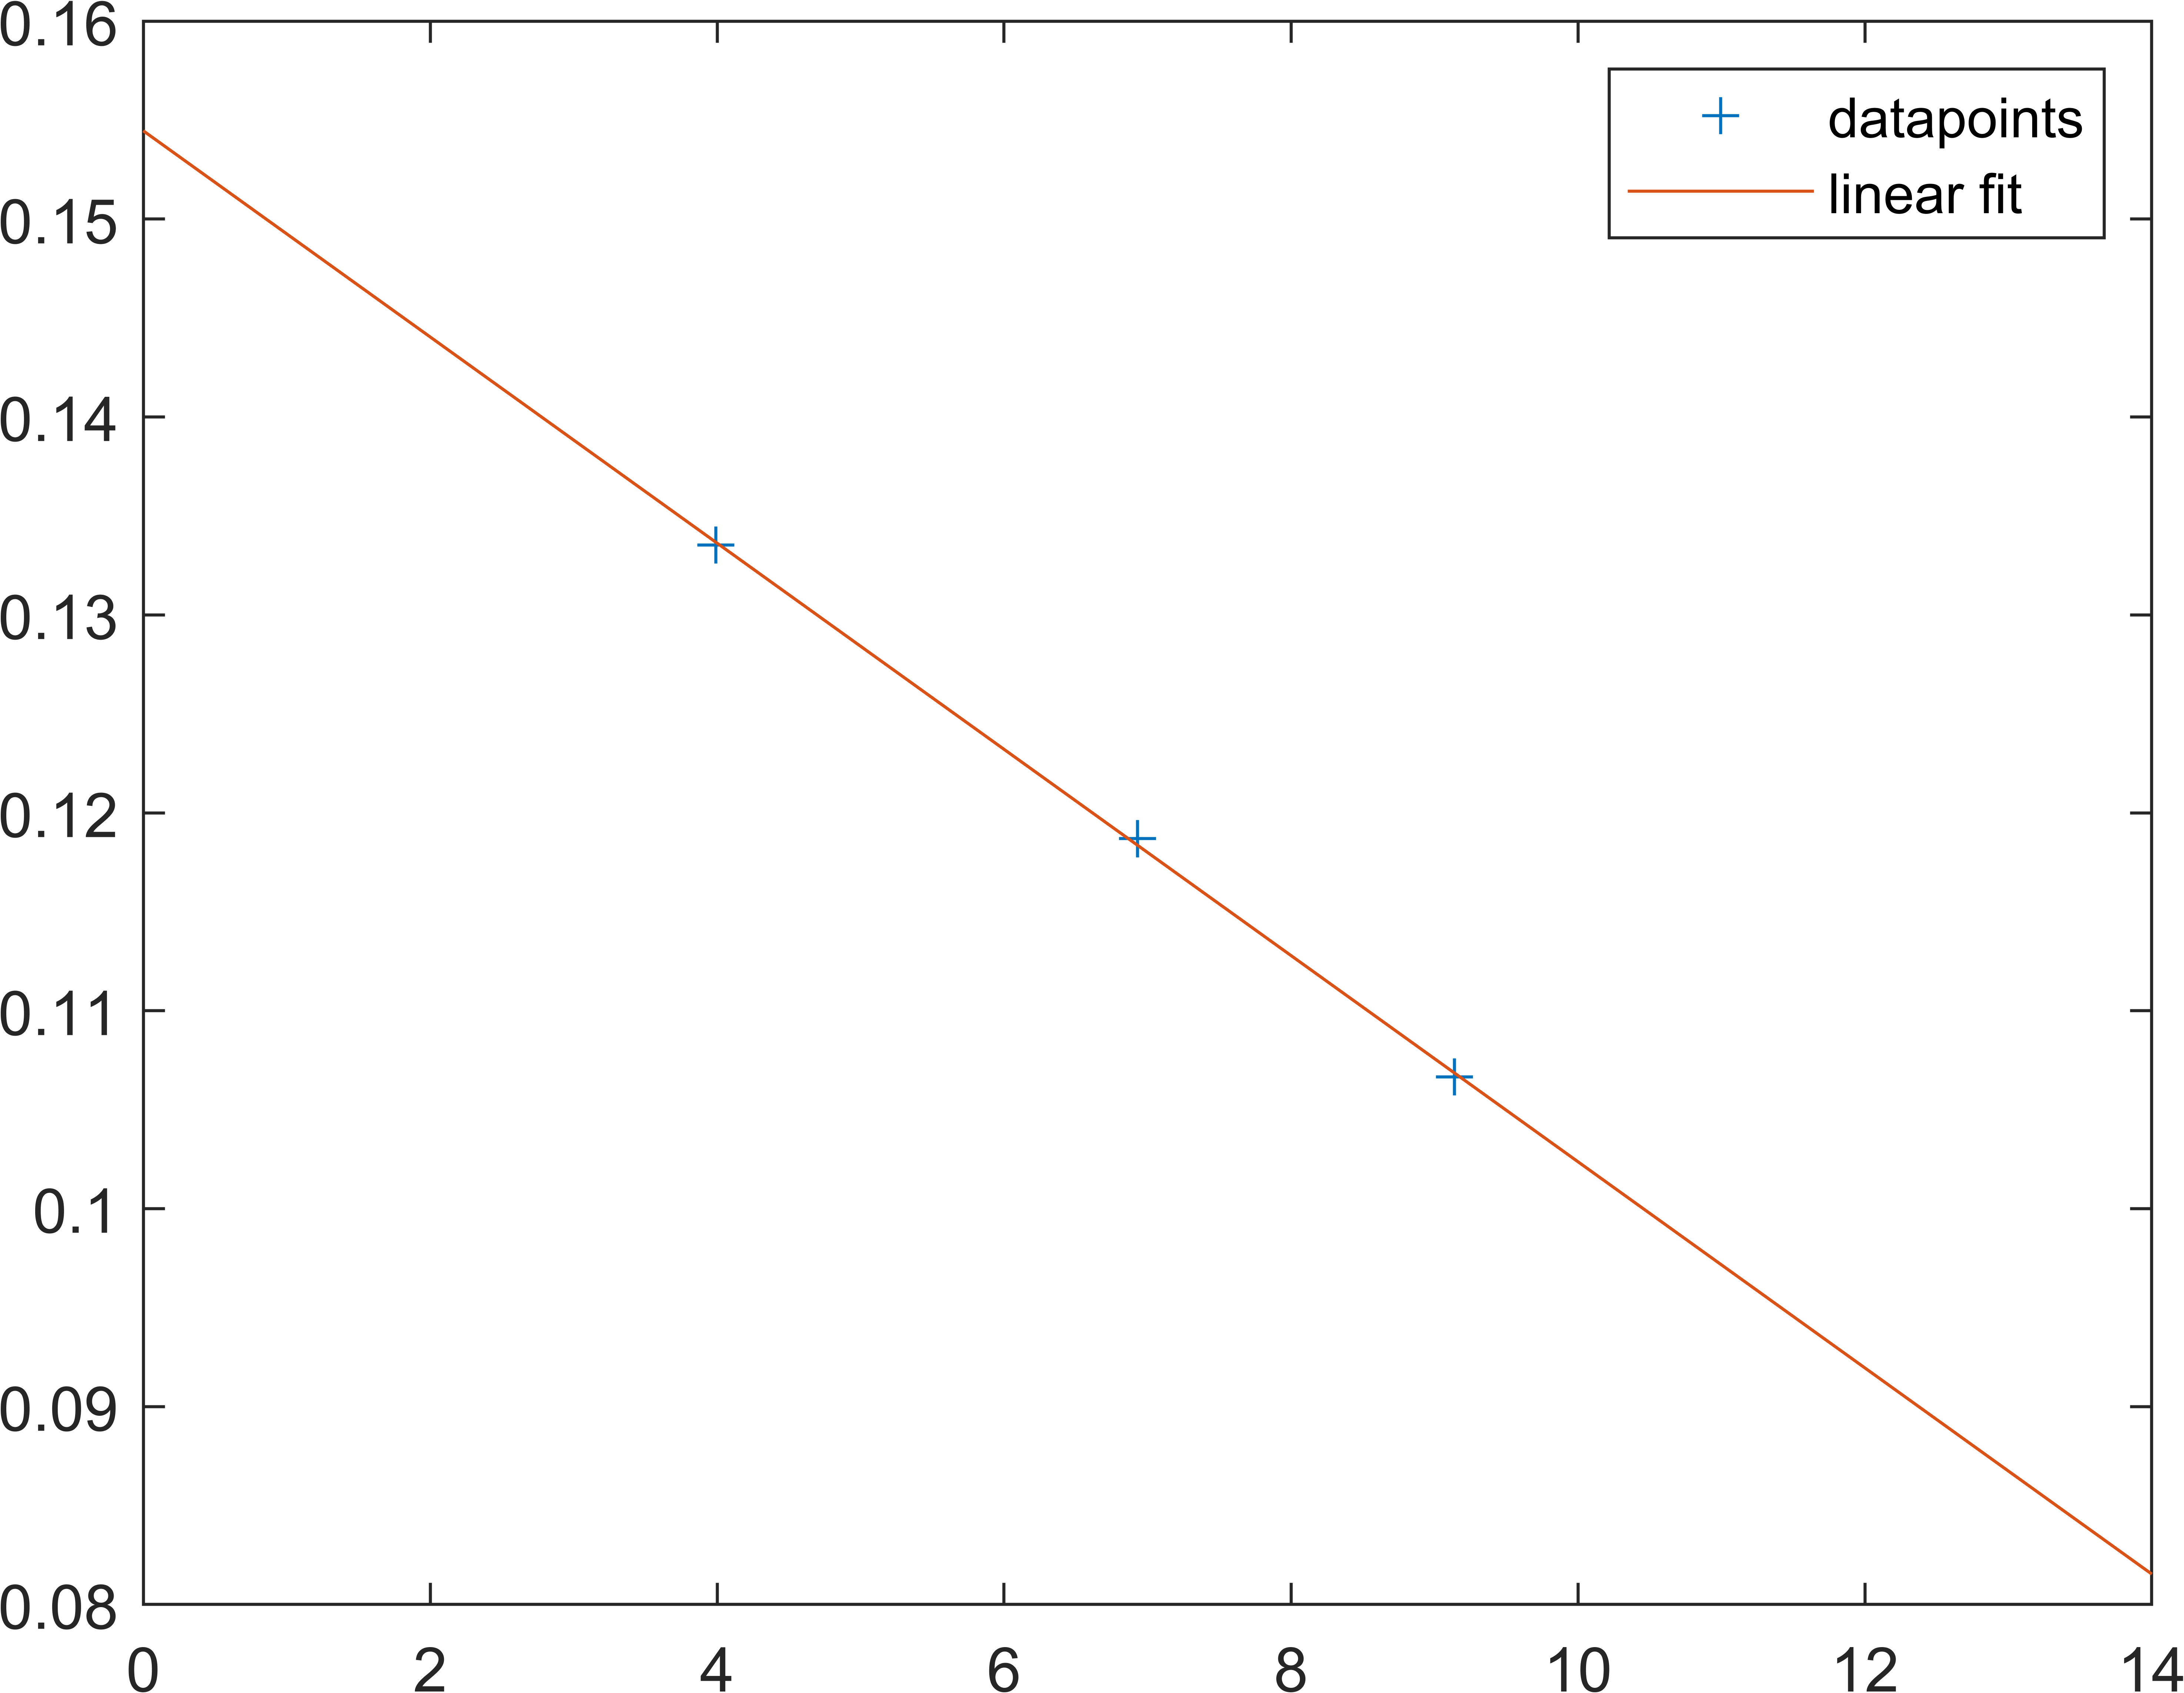
\includegraphics[width=0.8\linewidth]{src/images/phCalibrationGraph.png}
    \caption{Electrode voltage vs PH interpolation}
    \label{fig: phCalibrationGraph}
\end{figure}

\begin{figure}[H]
    \centering
    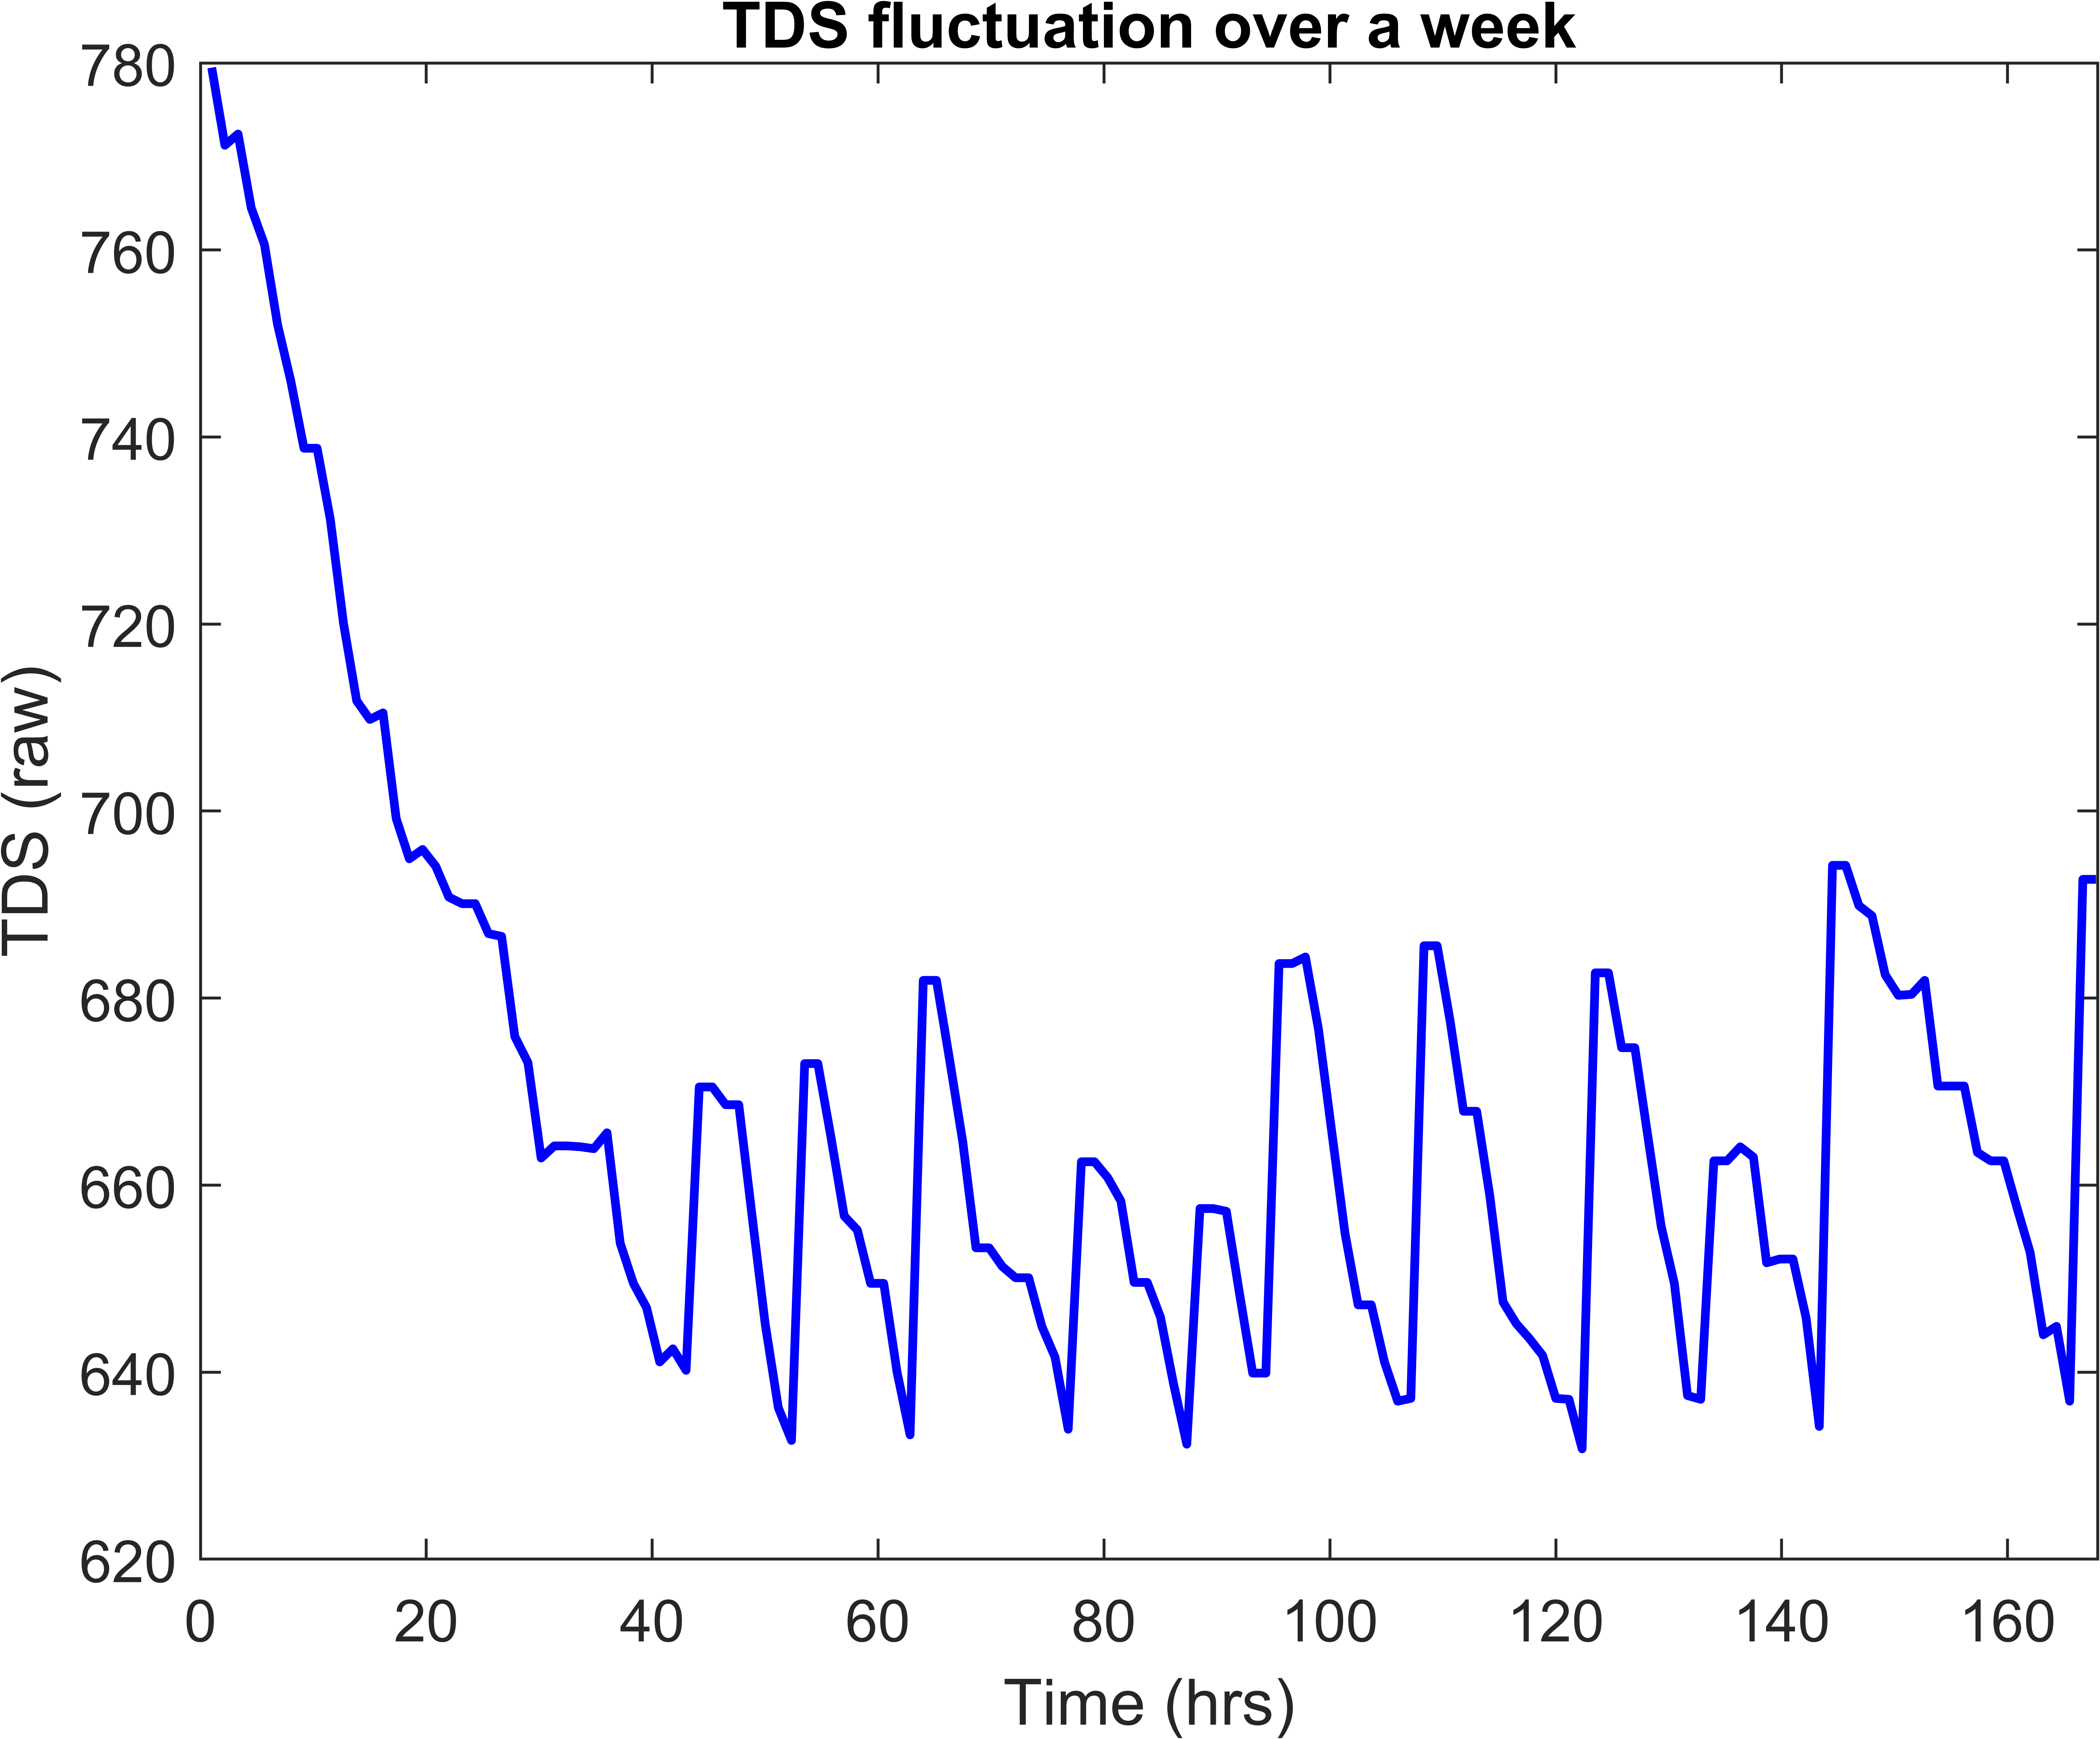
\includegraphics[width=0.8\linewidth]{src/images/tdsGraph.png}
    \caption{TDS Fluctuation Graph over a week}
    \label{fig: tdsGraph}
\end{figure}
The graph above displays the TDS fluctuation over a 1 week time period showing two distinct phases of behavior. During the first 40 hour mark a steep continuous decline is observed from approximately 780 units down to 640 units, representing a drop of roughly 140 units before the first dosing correction event occurs. The decline is slightly steeper than the expected 60 to 70 units drop per day for mature stages of lettuce, and is attributed to the initial TDS value being in the higher quarter of the threshold range. From 40 hours onward, a sawtooth oscillation can be observed between the ranges of approximately 630 to 690 units, demonstrating the activation of the nutrient dosing pump to compensate for the decline caused by plant uptake and evaporation. Each dosing event produces an abrupt upward correction of approximately 30 to 60 units, followed by a gradual decline as nutrients are consumed. The system successfully prevents TDS from falling below the minimum threshold of 560 units throughout the observation period.


\begin{table}[H]
\centering
\caption{System performance vs benchmark targets}
\label{tab:PerformanceComparison}
\renewcommand{\arraystretch}{1.4}
\begin{tabularx}{\textwidth}{|
>{\arraybackslash}L|
>{\arraybackslash}X|
>{\arraybackslash}X|
>{\arraybackslash}X|}
\hline
\textbf{S.N.} & \textbf{Performance Metric} & \textbf{Manual System (Reference)} & \textbf{Designed System}\\
\hline
1 & pH deviation ($\pm$ units)         & 0.6--1.2   & 0.30--0.38\\
\hline
2 & EC deviation ($\pm$ ppm)           & 150--300   & 30--60\\
\hline
3 & Monitoring frequency               & 2--4×/day  & 144×/day\\
\hline
4 & pH correction time (min)           & 30--120    & 5--10 \\
\hline
5 & EC correction time (min)           & 30--120    & 5--10 \\
\hline
6 & Human labour (h/week)              & 4--8       & $\sim$0.3\\
\hline
7 & Sensor accuracy -- pH ($\pm$)      & $\pm$0.2 typical & $\pm$0.1\\
\hline
8 & Sensor accuracy -- TDS (\%)        & $\pm$5\% typical & $\pm$2.5\%\\
\hline
\end{tabularx}


\end{table}


\begin{figure}[H]
    \centering
    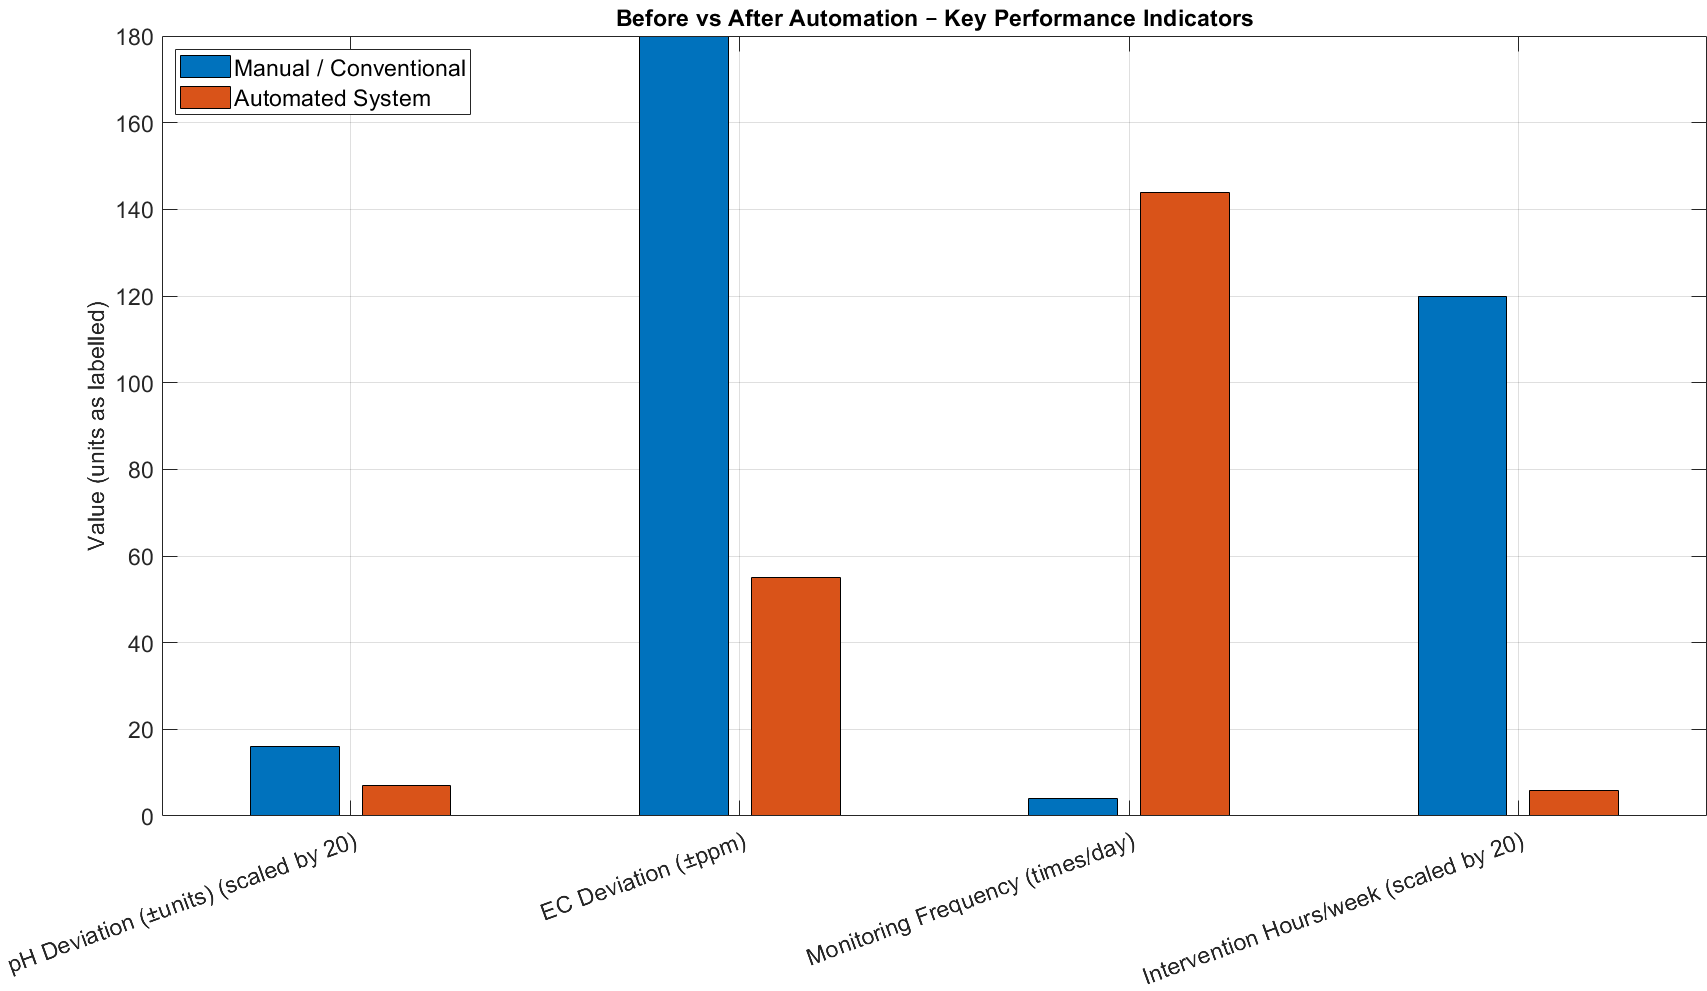
\includegraphics[width=1\linewidth]{src/images/IndicatorGraph.png}
    \caption{Before vs After Automation -- Performance Comparison}
    \label{fig: performanceGraph}
\end{figure}

The bar chart compares the performance of the manual conventional hydroponic system against the designed framework across four key indicators. In terms of pH deviation, the automated system reduced variation from $\pm$0.8 units to $\pm$0.35 units, demonstrating tighter nutrient solution control. EC deviation saw a similarly significant improvement, dropping from ±180 ppm under manual management to $\pm$55 ppm with automation, keeping nutrient concentration far closer to the crop-specific setpoint. Monitoring frequency increased dramatically from just 4 checks per day in a manual setup to 144 checks per day with the automated system, enabled by the 10-minute interval. Finally, operator intervention was reduced from approximately 6 hours per week to just 0.3 hours per week, with the remaining time attributed solely to periodic sensor recalibration. Across all four metrics, the automated approach demonstrates a clear improvement over manual operation, validating the effectiveness of the closed-loop control architecture for small-scale hydroponic cultivation.

\begin{figure}[H]
    \centering
    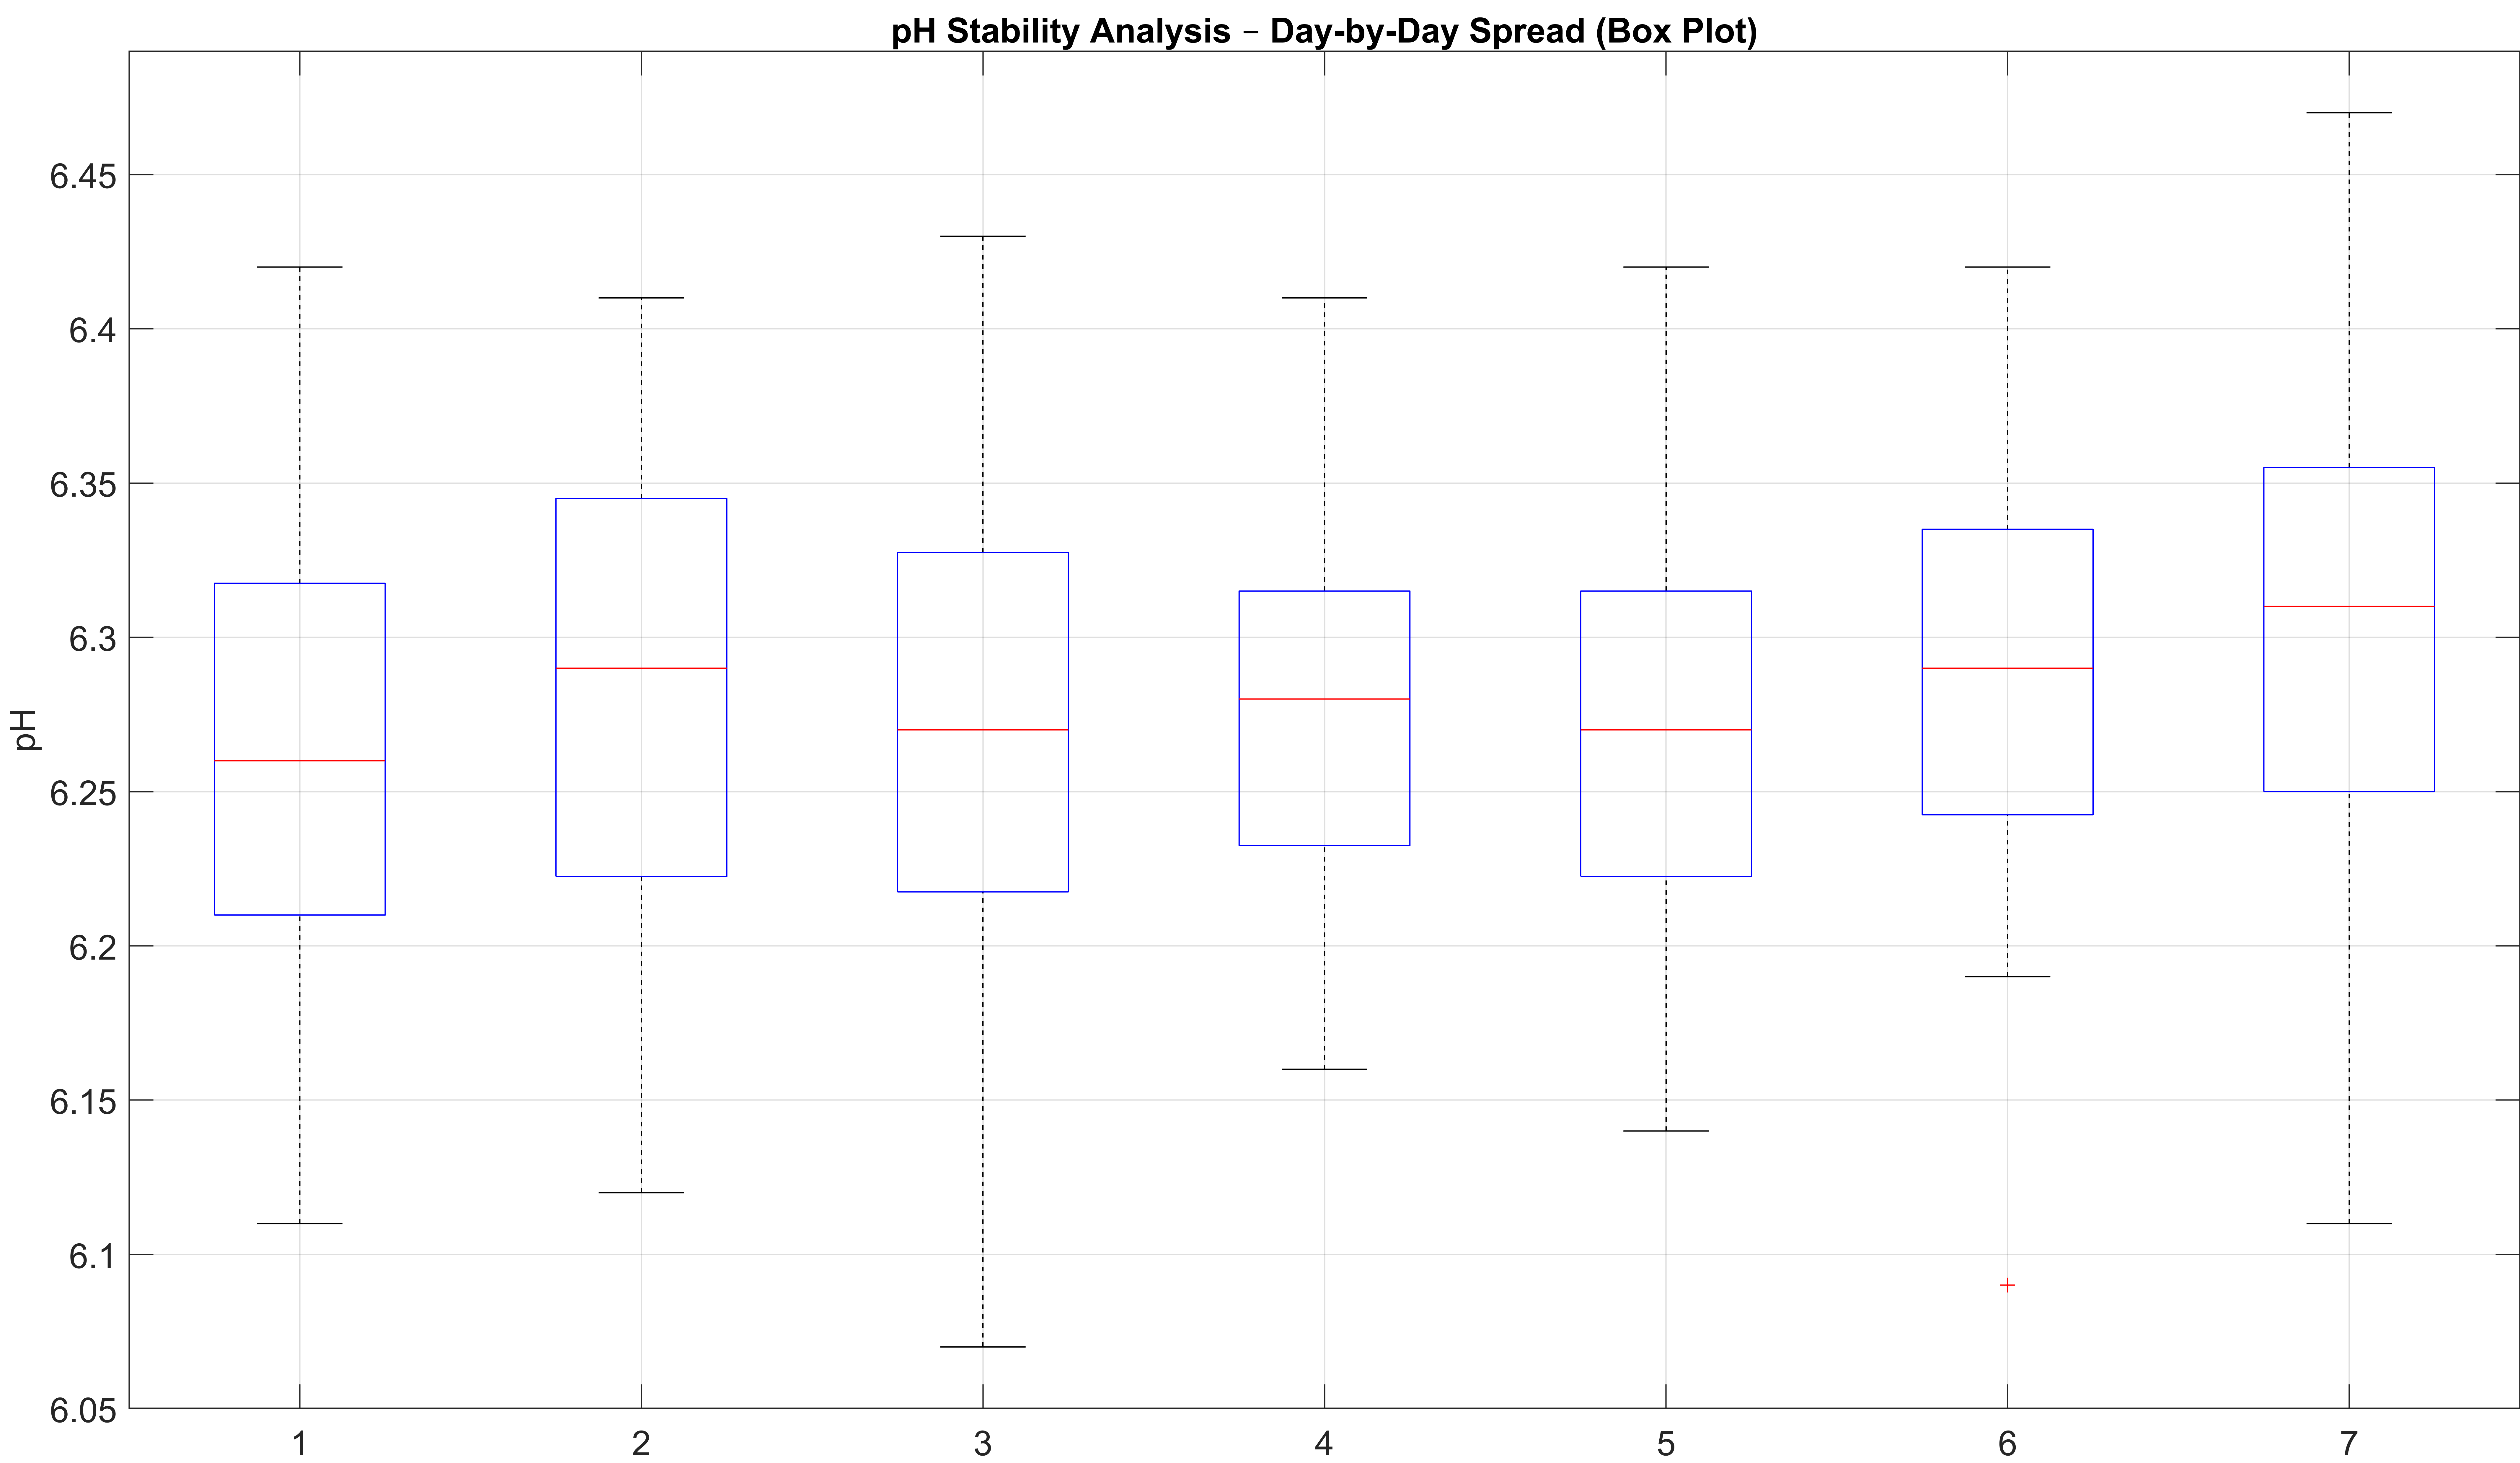
\includegraphics[width=1\linewidth]{src/images/phBoxPlot.png}
    \caption{pH stability daily box plot distribution over a week}
    \label{fig: phBoxPlot}
\end{figure}